16. Graph the equation below.
$$ quadraticGraphToEquationA $$ 
General Comments: Remember that Vertex Form is $y = a(x-h)^2+k$, where the vertex is $(h, k)$.

-----------------------------------------------

16. Graph the equation below.
$$ quadraticGraphToEquationA $$ 
The solution is  
 \begin{center} 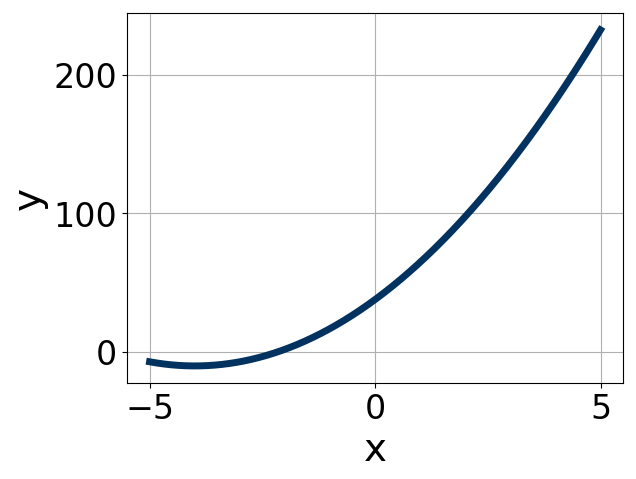
\includegraphics[width=0.5	extwidth]{../Figures/quadraticEquationToGraphBA.png} \end{center}\begin{tabular}{|c|c|} 
\hline 
 & \\ 
\textbf{A.} 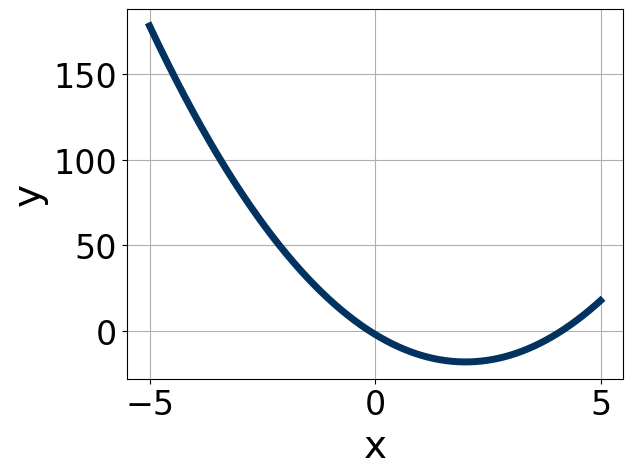
\includegraphics[width=0.5	extwidth]{../Figures/quadraticEquationToGraphAA.png} & \textbf{B.} 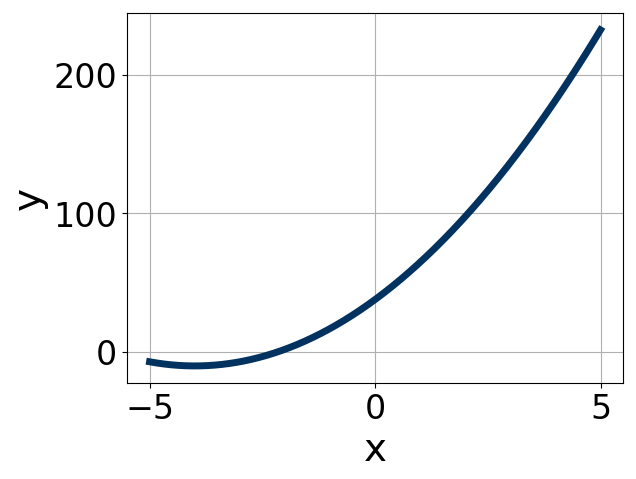
\includegraphics[width=0.5	extwidth]{../Figures/quadraticEquationToGraphBA.png} \\ 
\hline 
 & \\ 
\textbf{C.} 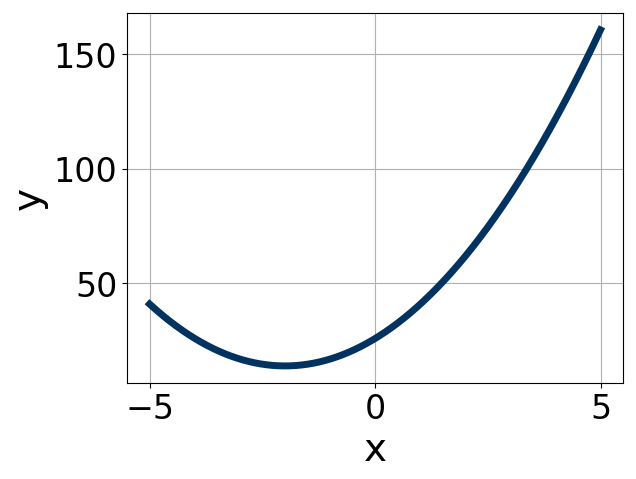
\includegraphics[width=0.5	extwidth]{../Figures/quadraticEquationToGraphCA.png} & \textbf{D.} 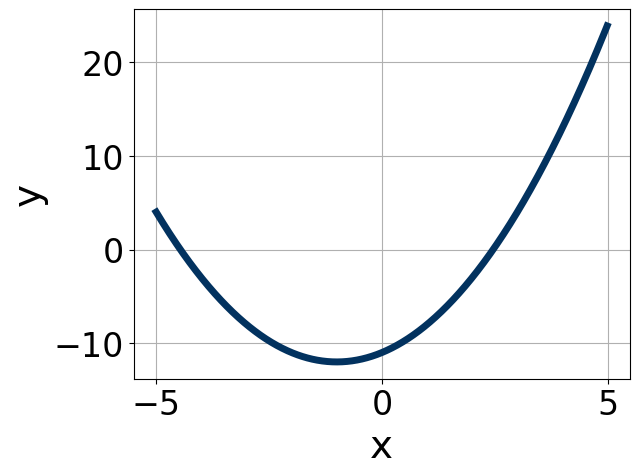
\includegraphics[width=0.5	extwidth]{../Figures/quadraticEquationToGraphDA.png} \\ 
\hline 
 & \\ 
 \textbf{E.} 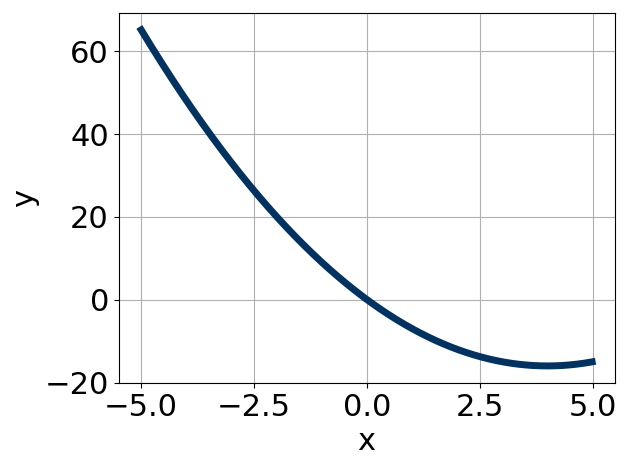
\includegraphics[width=0.5	extwidth]{../Figures/quadraticEquationToGraphEA.png} & \\ 
\hline 
 \end{tabular} 
 
General Comments: Remember that Vertex Form is $y = a(x-h)^2+k$, where the vertex is $(h, k)$.

-----------------------------------------------

16. Graph the equation below.
$$ f(x) = -(x-2)^2 + 13 $$ 
The solution is  
 \begin{center} 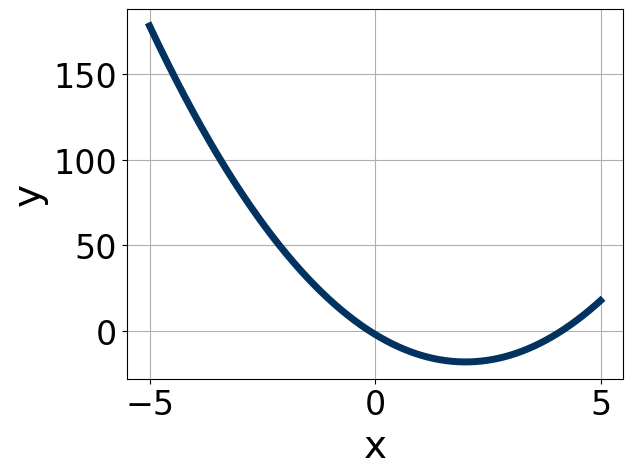
\includegraphics[width=0.5	extwidth]{../Figures/quadraticEquationToGraphAA.png} \end{center}\begin{tabular}{|c|c|} 
\hline 
 & \\ 
\textbf{A.} 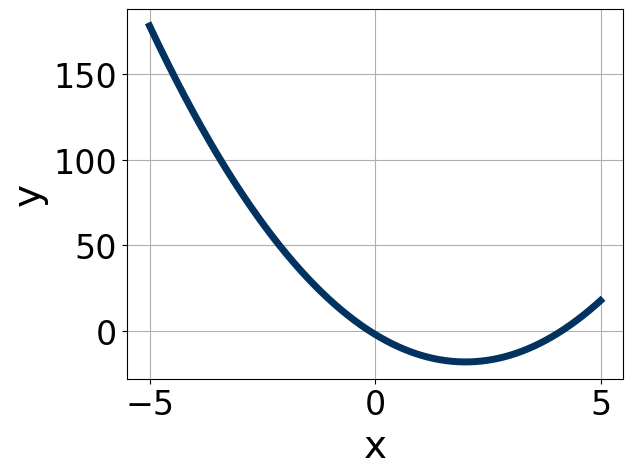
\includegraphics[width=0.5	extwidth]{../Figures/quadraticEquationToGraphAA.png} & \textbf{B.} 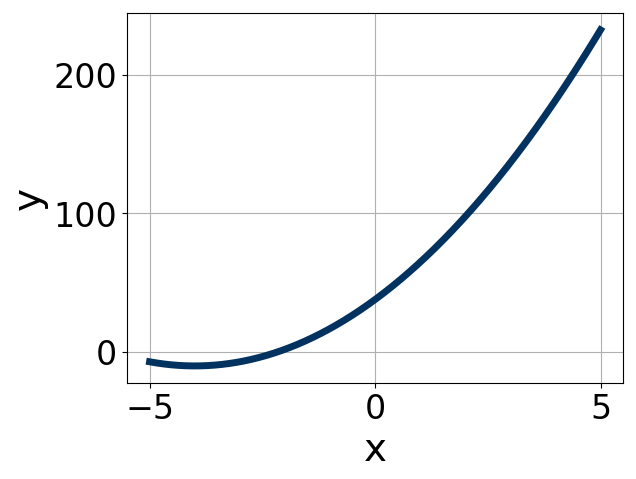
\includegraphics[width=0.5	extwidth]{../Figures/quadraticEquationToGraphBA.png} \\ 
\hline 
 & \\ 
\textbf{C.} 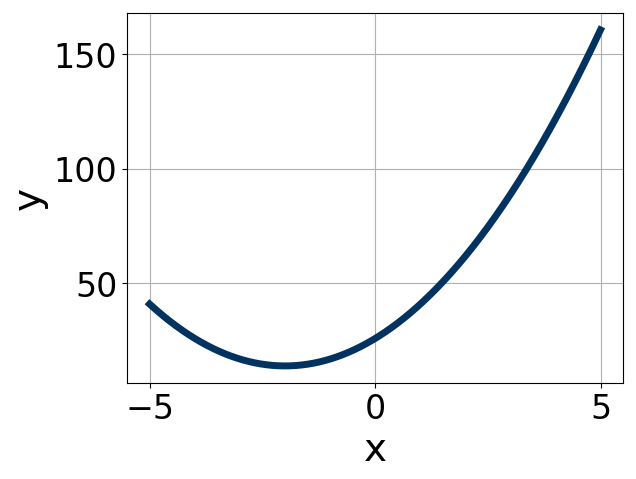
\includegraphics[width=0.5	extwidth]{../Figures/quadraticEquationToGraphCA.png} & \textbf{D.} 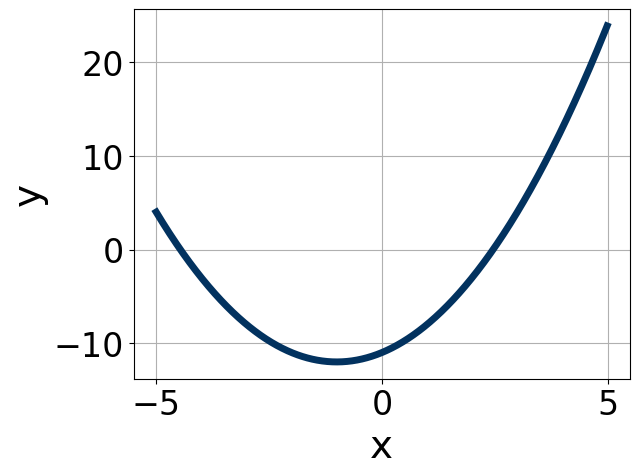
\includegraphics[width=0.5	extwidth]{../Figures/quadraticEquationToGraphDA.png} \\ 
\hline 
 & \\ 
 \textbf{E.} 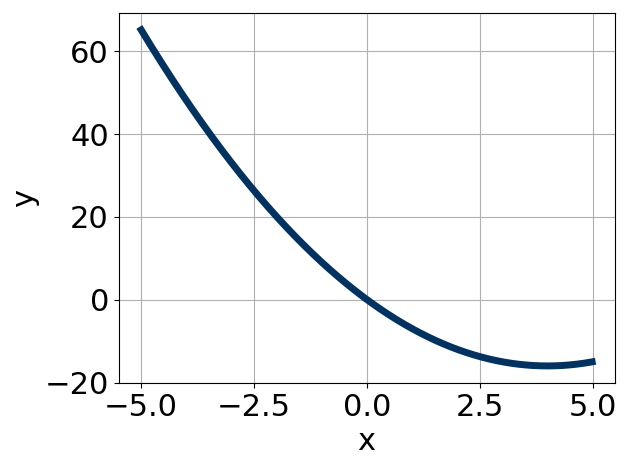
\includegraphics[width=0.5	extwidth]{../Figures/quadraticEquationToGraphEA.png} & \\ 
\hline 
 \end{tabular} 
 
General Comments: Remember that Vertex Form is $y = a(x-h)^2+k$, where the vertex is $(h, k)$.

-----------------------------------------------

